\chapter{UI \& UX Design} \label{chapter4}

No matter what functionalities we choose to employ in our news aggregator module, we need to build towards an interface that should be usable and easy to pick up regardless of the degree of a user's experience with the rest of the existing app. The new module should blend seamlessly with the current design and aim to complement the other functionalities of the app. We need to follow not only existing design guidelines in the app, but guidelines that are generally followed and predictable in several other modern apps. 

~
Following the results of our previous user study \textbf{\ref{3:results}}, we will discuss in this chapter the core user-facing functionalities of our module and the general framework that influenced our design choices. For prototyping, we used \textit{Figma}\footnote{https://www.figma.com/}, a powerful online tool for sketching, and in this chapter, we will describe the iterative process that led from our initial proposals to the final design of our module.

~

\section{General design} \label{4:general_design}

\textbf{ACS UPB Mobile} is a cross-platform app developed using the Flutter framework from Google\footnote{https://flutter.dev/}. From a single code base, Flutter compiles our app to native code for Android, iOS and web, but being able to run an app on a platform and having it look according to industry standards are two separate issues. Therefore, when discussing the general design framework for our current app, we have to understand what design guidelines and philosophies all these systems follow and what developers should be aware of when adapting an app from one platform to another.

~
Android apps generally follow the Material Design principles\footnote{https://material.io/design}, an adaptive set of guidelines and tools introduced by Google at Google I/O 2014 \cite{googleio_material}. According to their official documentation\footnote{https://material.io/archive/guidelines/layout/principles.html}, this framework \textit{"is guided by print-based design elements...to create hierarchy, meaning, and focus that immerse the user in the experience"}. On the other hand, iOS apps follow the Apple Human Interface Guidelines\footnote{https://developer.apple.com/design/human-interface-guidelines/guidelines/overview/}, a set of official principles that apps must adhere to when published to the App Store. Fortunately, to make it easier for developers, Flutter offers them a wide range of out-of-the-box widgets they could use for each platform, more specifically, Material\footnote{https://docs.flutter.dev/development/ui/widgets/material} widgets for Android and Cupertino\footnote{https://docs.flutter.dev/development/ui/widgets/cupertino} components for iOS. These widgets represent standard components that adhere to each framework's guidelines from a visual and behavioural point of view. Such components are buttons, icons, loading indicators, and alert dialogues; the list is not exhaustive.

~
However, achieving a perfectly-native design for both platforms with one single code base is a thorough process, and it generally requires platform-aware widgets that adapt their design accordingly or separate implementations for different functionalities. \textbf{ACS UPB Mobile} design focuses mainly on the Material guidelines, and for our purpose, we designed our module to follow best this framework guidelines. Nevertheless, our end product will run smoothly on both Android and iOS devices.

~

\section{User functionalities}\label{4:user_functionalities}

Based on our results obtained from the user study, we selected a number of functionalities worth taking into consideration for our feature. To get a clear view of how we should further develop our UI/UX, we tried to understand how each individual feature would impact our overall module by assessing its importance and usage frequency. We employed a red routes matrix approach to plot the most critical paths and to understand which features would be a high priority for our news aggregator module to work and which features would be more redundant than helpful from a user point of view. 
~

\begin{figure}[ht]
    \centering
    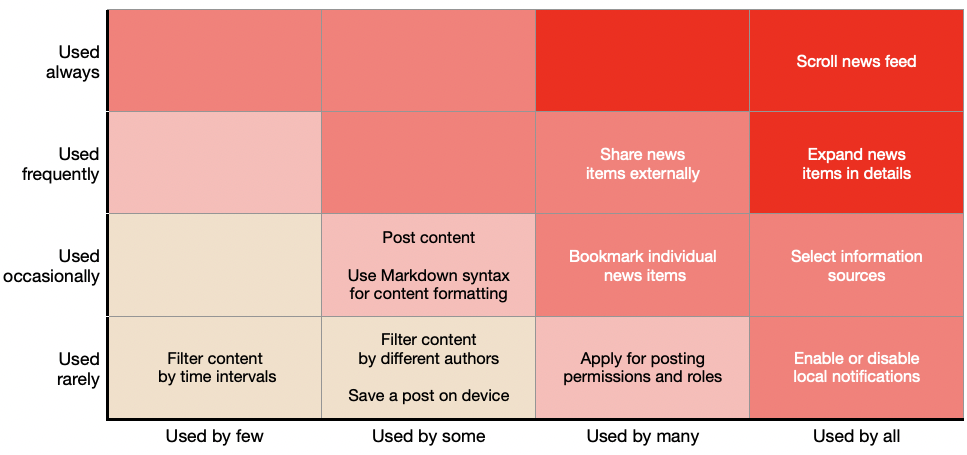
\includegraphics[width=\textwidth]{figures/app/miscellanous/red-routes-map.png}
    \caption{News aggregator red routes matrix}
    \label{3:fig:students_organizations}
\end{figure}

~
Unsurprisingly, the most crucial feature is having a main news feed page where users can scroll for their posts. Needless to say, this is the core functionality of our whole module, and therefore, it will be used by all users whenever they want to check for their news. Students will scroll the feed and see a relevant preview of each news item, and more than often, they will expand a particular post to read its entire content on a separate details page.

~
Regarding the social actions, following our user study, we concluded that actions such as liking or reporting a particular item do not bear any meaningful impact on our app. For example, liking a post does not influence a student's choice to view or not view an item they are interested in, whereas reporting a post is unnecessary since our information sources would be verified and, more or less, official. However, sharing externally a post is an excellent way to incentivise user traction and motivate other students to use the app. Sharing a dynamic link that sends a user to a specific item within our app would prove a common use case for our module.

~
Bookmarking is an essential ability for users to build their collection of favourite items. When considering this feature, we pondered the idea of letting users download their items locally on the device to have these posts available in both connected and offline mode. However, we concluded that while bookmarking an item may be an occasional action, downloading a post may be redundant for our app focus. For example, it is doubtful that a student would need to download a faculty post and access it at some point in offline mode. Moreover, we will employ Firebase services when building our module, which already do some local caching out-of-the-box.

~
Users should be required to select the information sources or enable their notifications before using the news feed. When logging into the app, users should immediately be prompted to perform these actions. Afterwards, they may occasionally resume to these settings to change something.

~
Even though students gave positive feedback on having sorting and filtering mechanisms, we concluded that these might not be so relevant for our news feed. It all comes down to our app's content load and users' need to revisit past posts. In practice, students would not resume that often to past news since such items mainly address present issues which are not that relevant in the long term. In other words, there would not be such posts that a user would feel the need to revisit after a long time. Moreover, the reduced frequency of updates would not hinder a user from scrolling directly to a post they are interested in from a few months ago, should that be the case.

~
Finally, there is a strong need to implement a role-based mechanism and administer which students have the right to post within our app. We wanted to give students the freedom to apply via an in-app form for such rights, and they should be aware of this possibility when using the news feed. We felt that our module should act as a content aggregator from different sources and simultaneously enable students to contribute with valuable posts for their colleagues. 

~
As \textbf{Ioana Alexandru} described in her thesis \cite{ioana-alexandru-permission-levels}, \textbf{ACS UPB Mobile} employs different permission levels that control which actions a user can do within the app. The highest level is reserved for just a handful of admin users, who accept or decline permission requests, and below them is the group of users that can add or edit public information. Students must be given these editing permissions beforehand whenever they want to post content. Additionally, since these students might hold one or more official titles in their collective, we want to give them the possibility of having separate roles within our app. For example, a student that is both president of a student association and a representative in the Faculty Council might hold two roles. Ultimately, these roles should help students better place their posts in the right information source category. Students might post on behalf of the faculty, of a student organization, or themselves; therefore, all posts coming from students should not be placed by default in the same information source category. We will further explain our role-based approach in \textbf{chapter \ref{chapter5}}.

~
Although users may not post frequently, this is an essential feature we want to employ for our module. Enabling \textbf{Markdown syntax}\footnote{https://www.markdownguide.org/basic-syntax/} formatting would help students personalize and design their posts more attractively, so we 
were confident this would be a feature that they would use.

~
Summing up, this is how we trimmed down our initial features list to the one described in the proposed functionalities section \textbf{\ref{1:functionalities}}. Again, we tried to take user feedback into account and we tried to understand what our news feed module focus will be. 

~

\section{General user workflow} \label{4:general_user_workflow}

\subsection{User stories} \label{4:user_stories}

The following user stories reflect how users should interact with different parts of our module. We distinguish between three types of accounts: regular \textbf{User} with no publishing rights, \textbf{Editor} with both publishing rights and roles, and \textbf{Admin} with supreme rights. For clarification, every Editor is a User, but not every User is an Editor. An Admin is both User and Editor.

~

\textbf{As a User:}
\begin{itemize}
    \setlength{\topsep}{0.5pt}
    \setlength{\itemsep}{0.5pt}
    \setlength{\parsep}{0.5pt}
    \item I want to scroll my news items from a centralized feed page.
    \item I want to have main categories for my news, such as All or Favorites.
    \item I want to bookmark a post, so that I can revisit it in my Favorites category.
    \item I want to share a post externally via URL.
    \item I want to select my information sources, so that I receive filtered content.
    \item I want to choose to enable or disable notifications for news updates.
    \item I want to be able to apply for editing permissions, so that I can become an Admin and start publishing content.
\end{itemize}

~

\textbf{As an Editor:}
\begin{itemize}
    \setlength{\topsep}{0.5pt}
    \setlength{\itemsep}{0.5pt}
    \setlength{\parsep}{0.5pt}
    \item I want to be able to apply for posting roles, so that I can have different posting titles.
    \item I want to be able to compose a new post.
    \item When I compose a post, I want to be able to choose a specific target group and posting role.
\end{itemize}

~

\textbf{As an Admin:}
\begin{itemize}
    \setlength{\topsep}{0.5pt}
    \setlength{\itemsep}{0.5pt}
    \setlength{\parsep}{0.5pt}
    \item I want to accept or decline requests from both Users and Editors.
\end{itemize}

\subsection{Workflow diagram} \label{4:workflow_diagram}

To better illustrate how our news feed module and additional admin features will integrate with the rest of the present app workflow, we propose the following state diagram \textbf{\ref{4:fig:general_workflow}}. 

\begin{figure}[ht]
    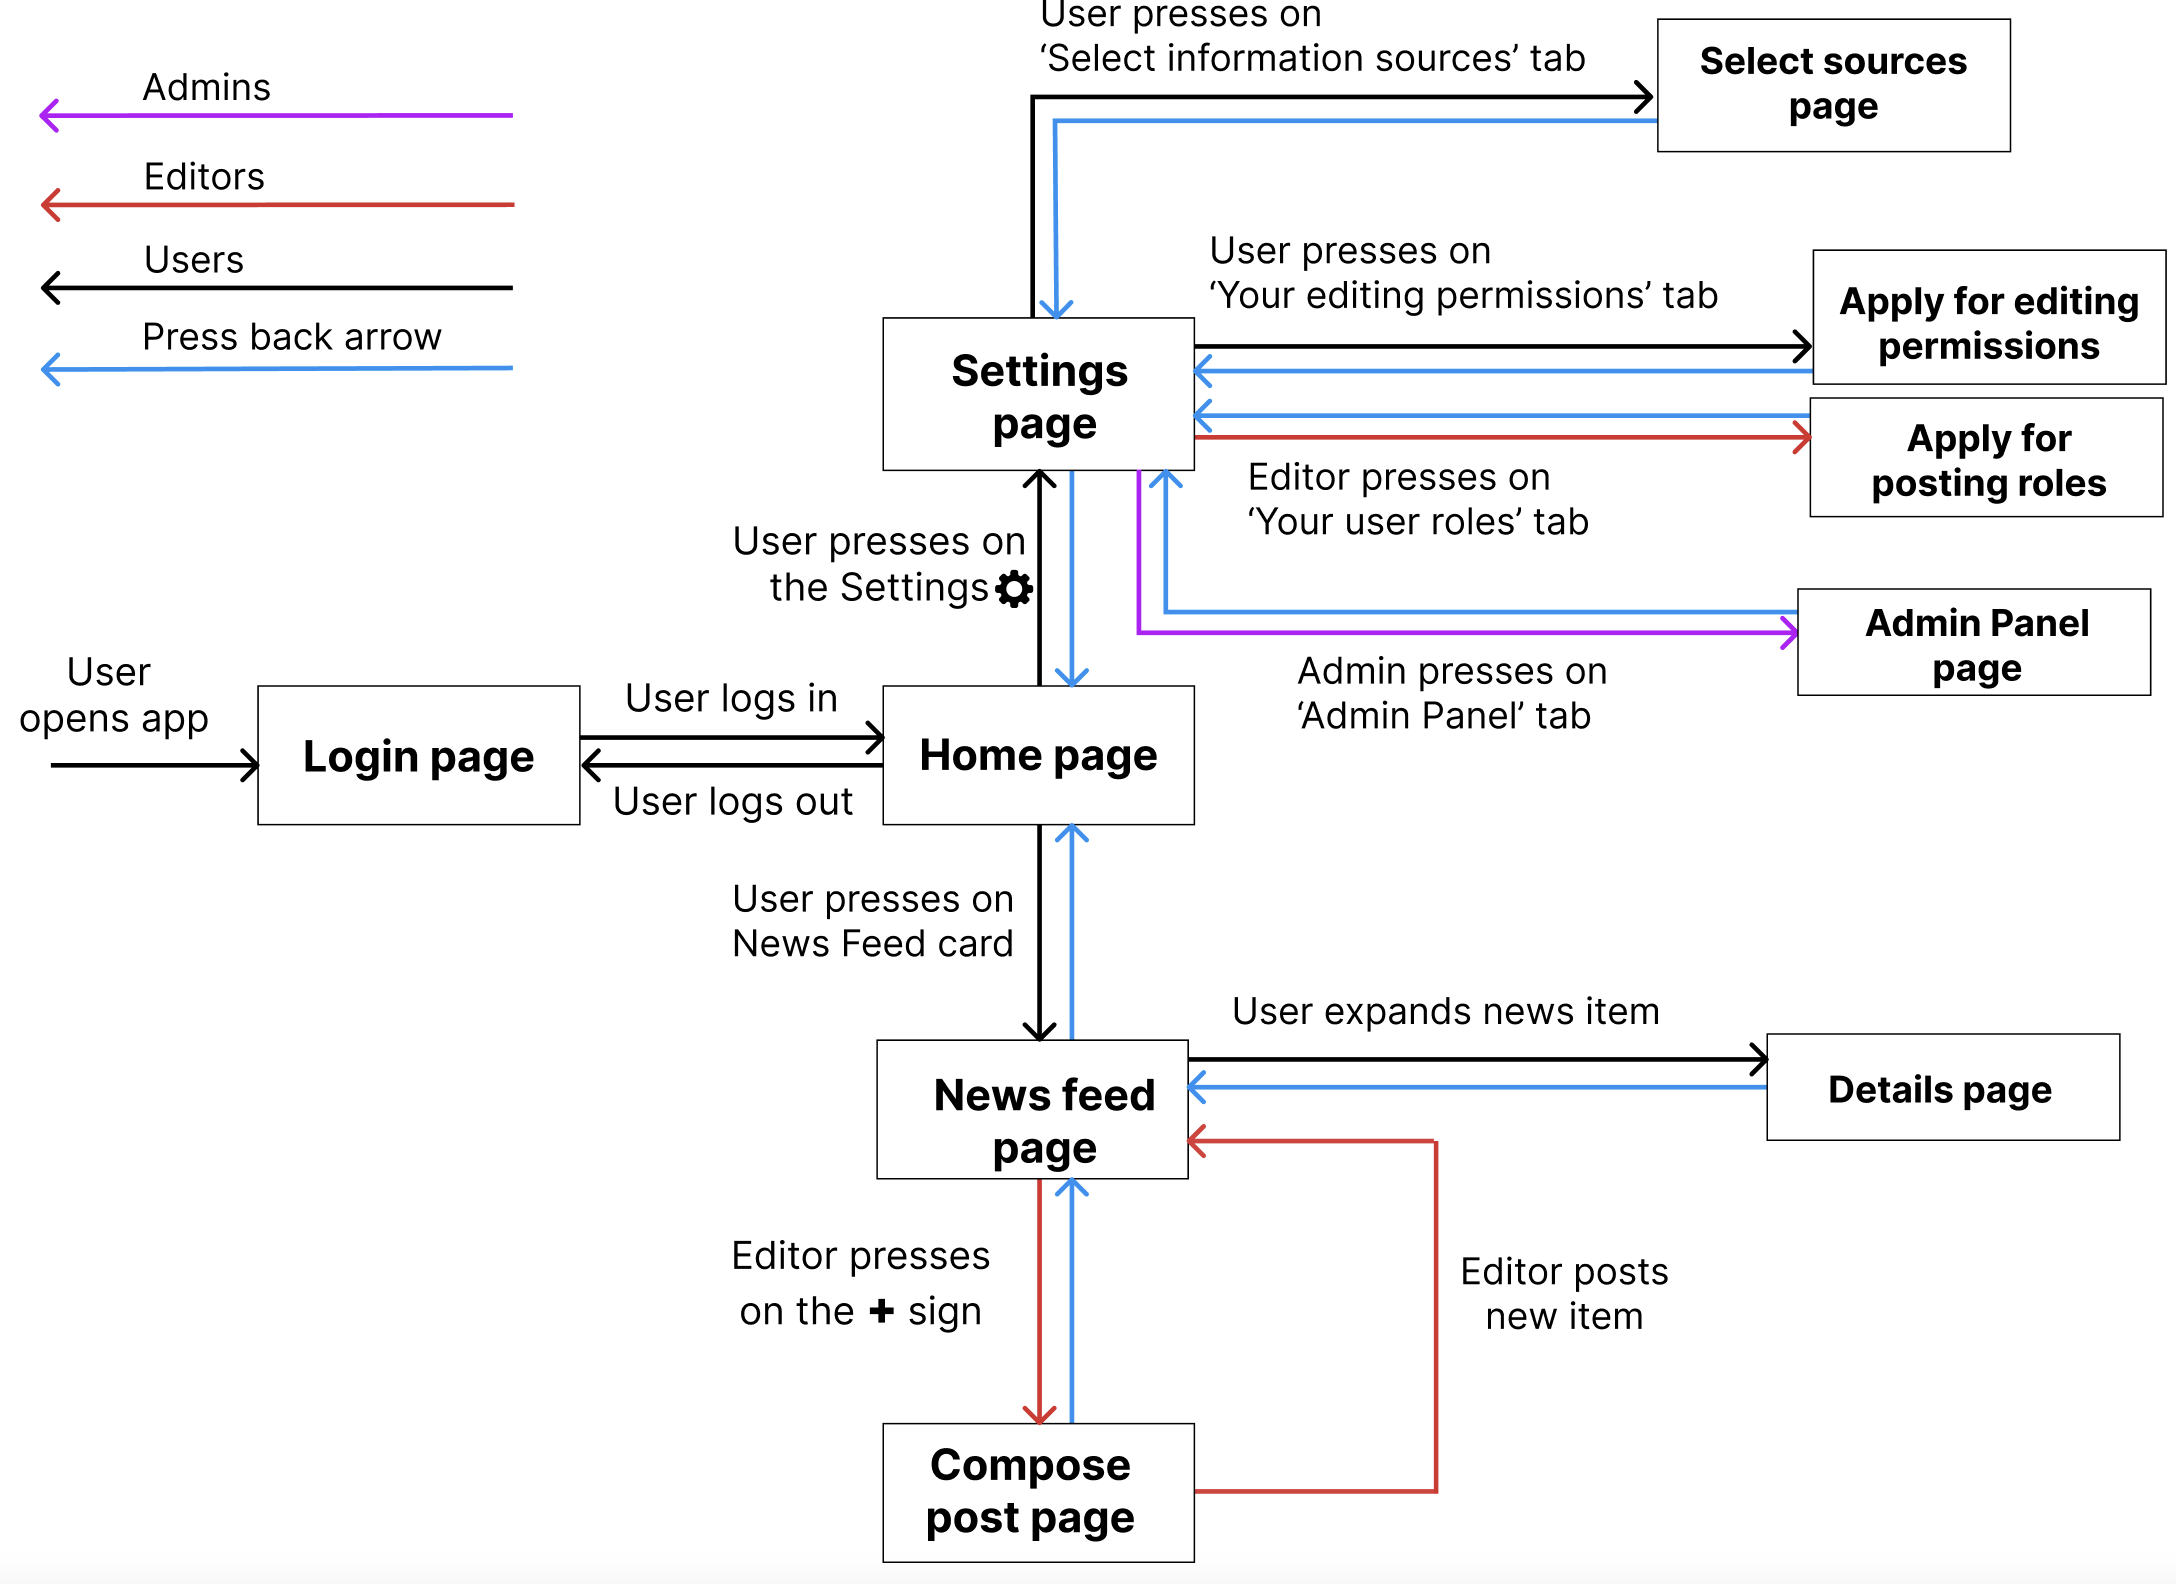
\includegraphics[width=\textwidth]{figures/app/miscellanous/general-user-workflow.png}
    \caption{General workflow diagram}
    \label{4:fig:general_workflow}
\end{figure}

\section{Prototyping} \label{4:prototyping}

With a list of relevant functionalities in mind, we started prototyping our design using \textbf{Figma}\footnote{https://www.figma.com/}. During the process, we tried to get a good grip on the design guidelines present in the \textbf{ACS UPB Mobile} app, and we worked in a close feedback loop with members of the contributing group. Our approach was more not to reinvent the wheel but try to reuse existing, proven functionalities and practices. Moreover, we try to have our new design not interfere with other critical paths in the app.


\subsection{Initial design} \label{4:initial_design}

For our initial design, we took inspiration from the current app design and tried sketching the main screen without emphasising the details. In addition, we tried to use icons, several text labels and and follow the app's colour theme.

\begin{figure}[!ht]
    \centering
    \begin{minipage}[t]{0.4\textwidth}
        \captionsetup{justification=centering}
        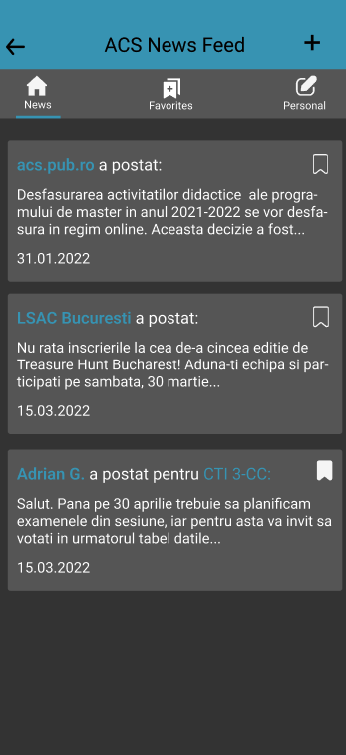
\includegraphics[width=\textwidth]{figures/app/initial/news-feed-draft.png}
        \caption{Draft news feed main page}
        \label{4:fig:draft-news-main-list-page}
    \end{minipage}
    \hfill
    \begin{minipage}[t]{0.4\textwidth}
        \captionsetup{justification=centering}
        
\includegraphics[width=\textwidth]{figures/app/initial/news-details-draft.png}
        \caption{Draft news details separate page}
        \label{4:fig:draft-news-details-page}
    \end{minipage}
\end{figure}

~
The main news feed page \textbf{\ref{4:fig:draft-news-main-list-page}} should have two or three big categories that could be accessed via a tab navigation bar: \textbf{News}, \textbf{Favorites} or \textbf{Personal}. The News category should list all available news items, whereas Favorites has the bookmarked ones and Personal has the posts that were composed by that user. Students will be shown the first two or all three categories, depending on their editing permissions. Each news item has a preview body, an author, a target group, a timestamp and a bookmark action, and when the user clicks on a specific item to expand it and is redirected to a separate details page. In addition, the main page has a plus icon in the top-right corner from where a student can compose a post.

~
The details page \textbf{\ref{4:fig:draft-news-details-page}} contains the entire post content and has two actions: bookmark and share. Moreover, whether a post was composed by the current user, we may choose to show a Trash icon so the user can delete the post if they choose.

\begin{figure}[!ht]
    \centering
    \begin{minipage}[b]{0.32\textwidth}
        \captionsetup{justification=centering}
        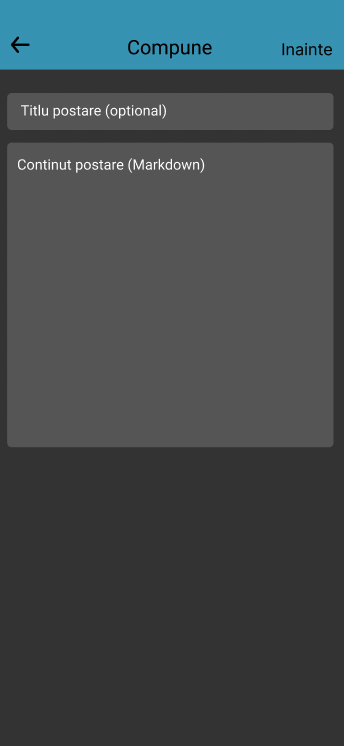
\includegraphics[width=\textwidth]{figures/app/initial/compose-step-1-draft.png}
        \caption{Draft compose post - content}
        \label{4:fig:draft-create-post-title-body}
    \end{minipage}
    \hfill
    \begin{minipage}[b]{0.32\textwidth}
        \captionsetup{justification=centering}
        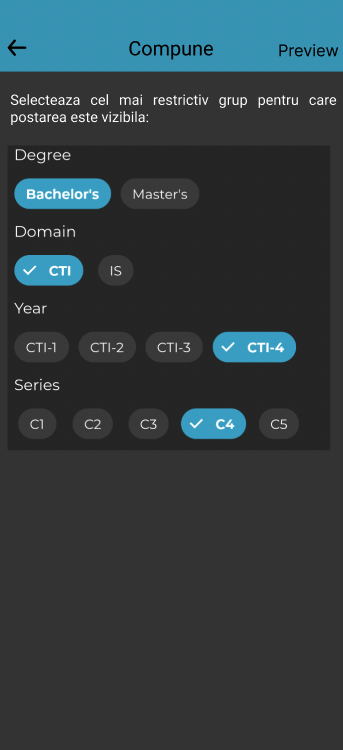
\includegraphics[width=\textwidth]{figures/app/initial/compose-step-2-draft.png}
        \caption{Draft compose post - relevance}
        \label{4:fig:draft-create-post-target}
    \end{minipage}
    \hfill
    \begin{minipage}[b]{0.32\textwidth}
        \captionsetup{justification=centering}
        
\includegraphics[width=\textwidth]{figures/app/initial/compose-step-3-draft.png}
        \caption{Draft compose post - preview}
        \label{4:fig:draft-create-post-preview}
    \end{minipage}
\end{figure}

\begin{figure}[!ht]
    \centering
    \begin{minipage}[t]{0.4\textwidth}
        \captionsetup{justification=centering}
        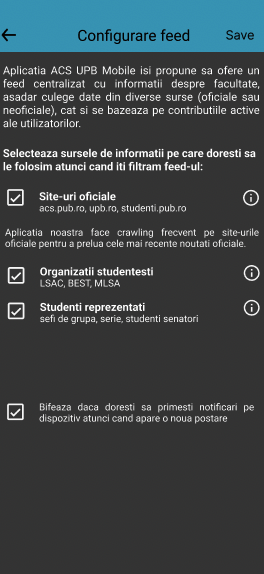
\includegraphics[width=\textwidth]{figures/app/initial/select-sources-draft.png}
        \caption{Draft select sources}
        \label{4:fig:draft-select-sources-page}
    \end{minipage}
    \hfill
    \begin{minipage}[t]{0.4\textwidth}
        \captionsetup{justification=centering}
        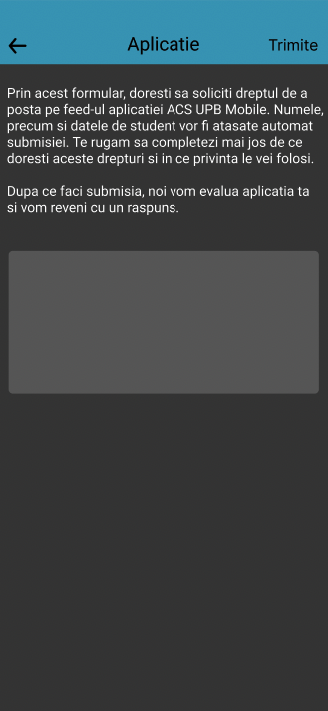
\includegraphics[width=\textwidth]{figures/app/initial/request-role-draft.png}
        \caption{Draft request roles}
        \label{4:fig:draft-request-roles-page}
    \end{minipage}
\end{figure}

We pondered on the idea of splitting the compose post action in multiple steps. Initially, the user chooses the title and body \textbf{\ref{4:fig:draft-create-post-title-body}}, then the target group \textbf{\ref{4:fig:draft-create-post-target}} or his role. Before publishing the post, they are shown a preview of the post \textbf{\ref{4:fig:draft-create-post-preview}} to make sure everything looks according to their intention. Later, in the final design, we dropped the idea of having multiple screens and we put everything on a single page to be consistent with the rest of the app.

~
The user configures their information sources from a separate screen \textbf{\ref{4:fig:draft-select-sources-page}}. For the moment, we provided three main sources: \textbf{Official}, \textbf{Student Organizations} and \textbf{Representative Students}. From the same screen, we wanted to give the user the possibility of enabling his notifications as well.

~
When requesting permissions or roles \textbf{\ref{4:fig:draft-request-roles-page}}, the user must fill in a form and, most importantly, specify a reason for his request. Requests will be handled separately by admins on a separate screen that is already present in the application.


\subsection{Final design} \label{4:final_design}

Starting from our initial design and our proposed functionalities, we arrived eventually at our final user interface.

\begin{figure}[!ht]
    \centering
    \begin{minipage}[b]{0.32\textwidth}
        \captionsetup{justification=centering}
        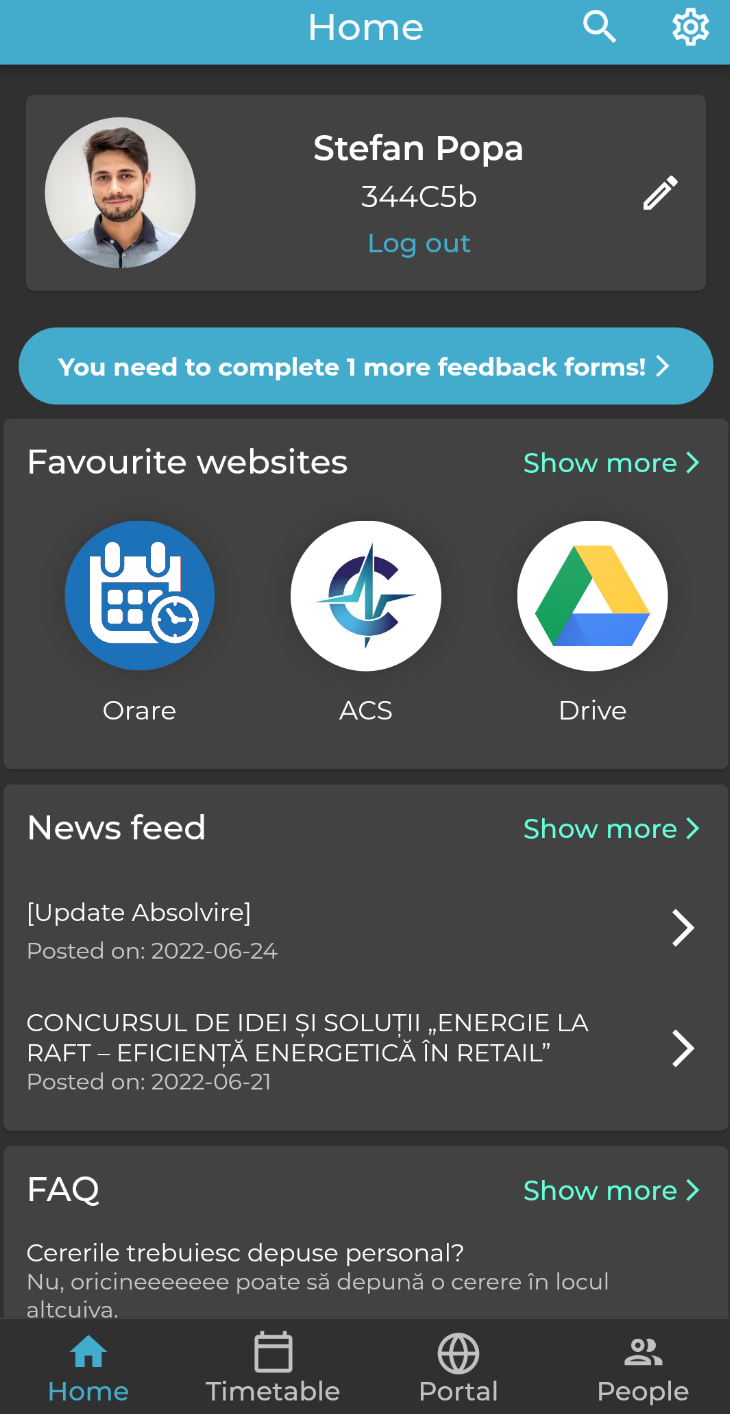
\includegraphics[width=\textwidth]{figures/app/final/home-page-final.png}
        \caption{News feed card on Home page}
        \label{4:fig:news-feed-home-page}
    \end{minipage}
    \hfill
    \begin{minipage}[b]{0.32\textwidth}
        \captionsetup{justification=centering}
        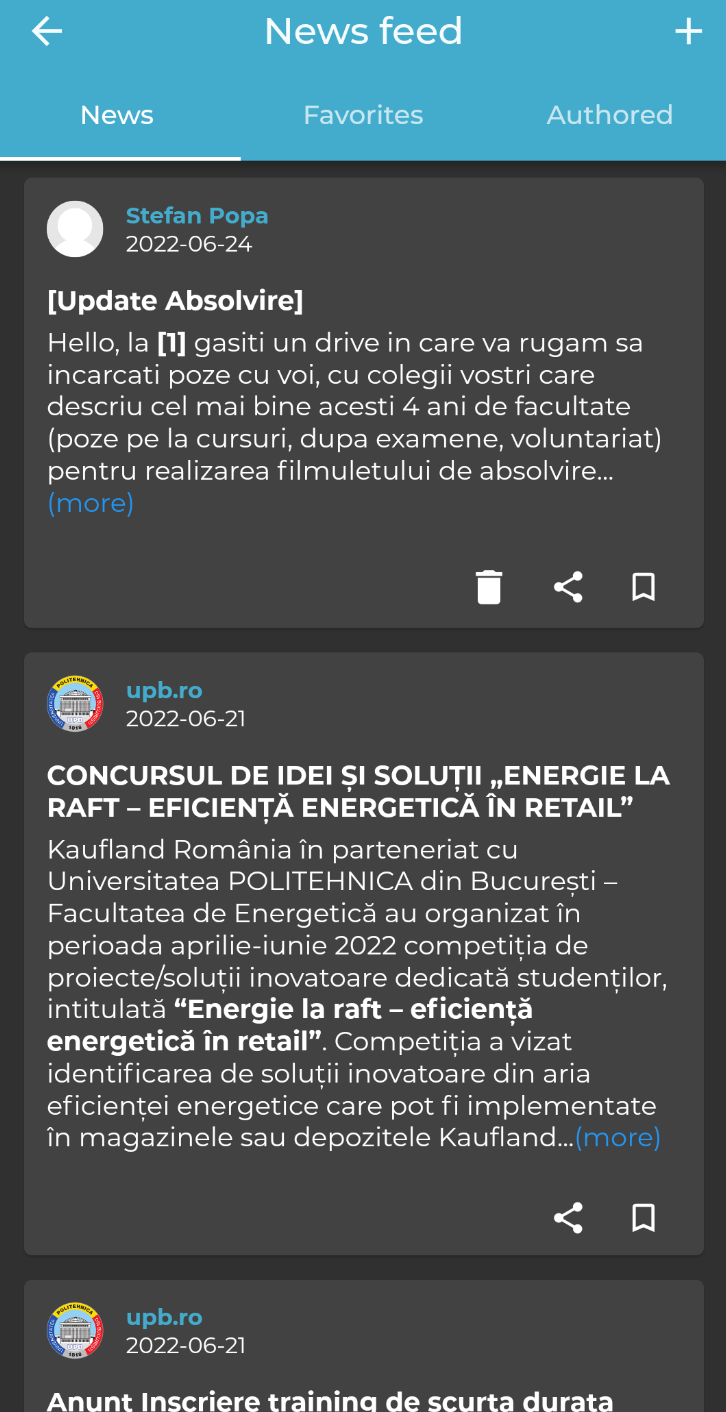
\includegraphics[width=\textwidth]{figures/app/final/news-feed-2-final.png}
        \caption{News feed main page}
        \label{4:fig:news-feed-final}
    \end{minipage}
    \hfill
    \begin{minipage}[b]{0.32\textwidth}
        \captionsetup{justification=centering}
        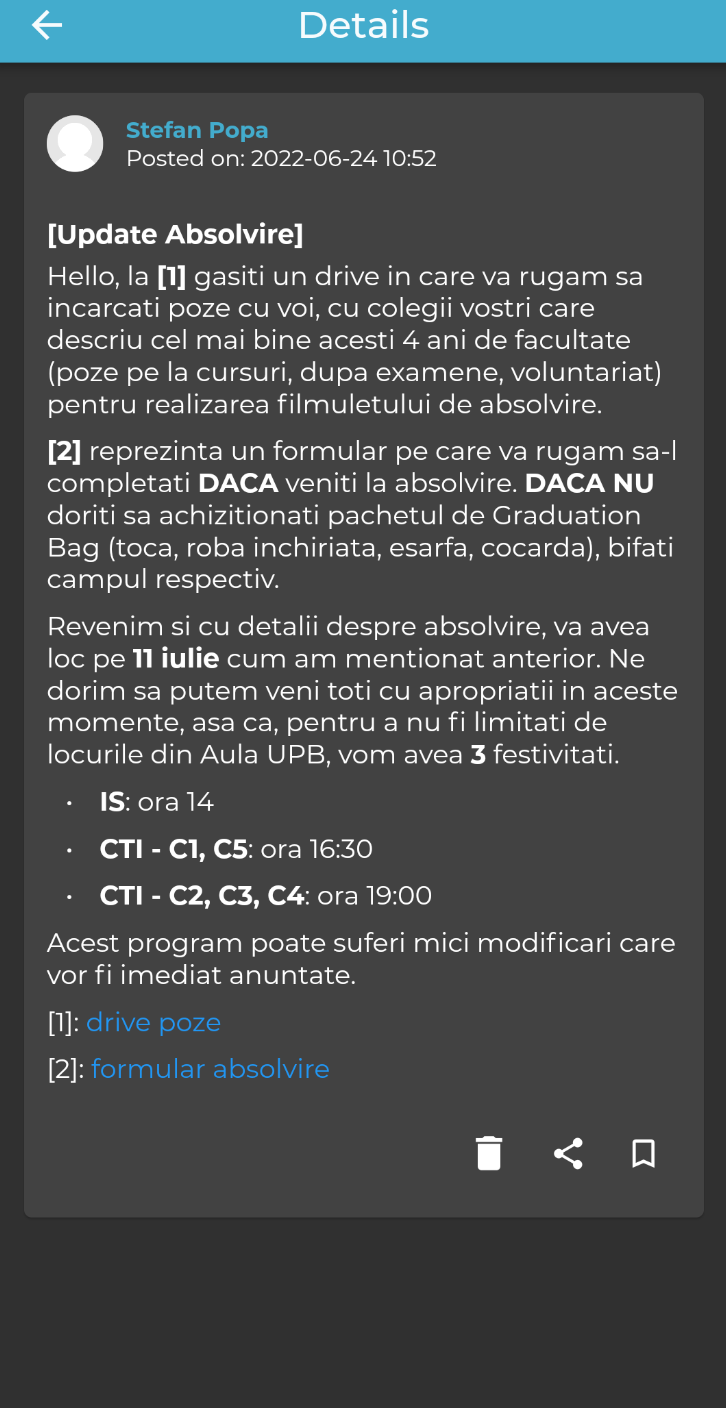
\includegraphics[width=\textwidth]{figures/app/final/news-details-final.png}
        \caption{News details separate page}
        \label{4:fig:news-details-final}
    \end{minipage}
\end{figure}

As described in our \textbf{Workflow diagram \ref{4:workflow_diagram}}, by the time the user logs in the app, they arrive on the Home page \textbf{\ref{4:fig:news-feed-home-page}}. They are presented with the news feed card that transitions them on click to the main news feed page \textbf{\ref{4:fig:news-feed-final}}. Our feed categories are: \textbf{News}, \textbf{Favorites} and \textbf{Authored} (the last category will be shown depending on whether the user has editing permissions). Users can navigate to the details page of a news item \textbf{\ref{4:fig:news-details-final}} when expanding it on click or opening it from a shared deep-link. Logged-in users can have multiple actions: bookmark, share or delete. The last option is enabled only if the current user is the author of that specific post. Bookmarked posts can be visualized in the favourites category on the main news feed page. Likewise, authored posts can be easily accessed from their according category.

\begin{figure}[!ht]
    \centering
    \begin{minipage}[b]{0.32\textwidth}
        \captionsetup{justification=centering}
        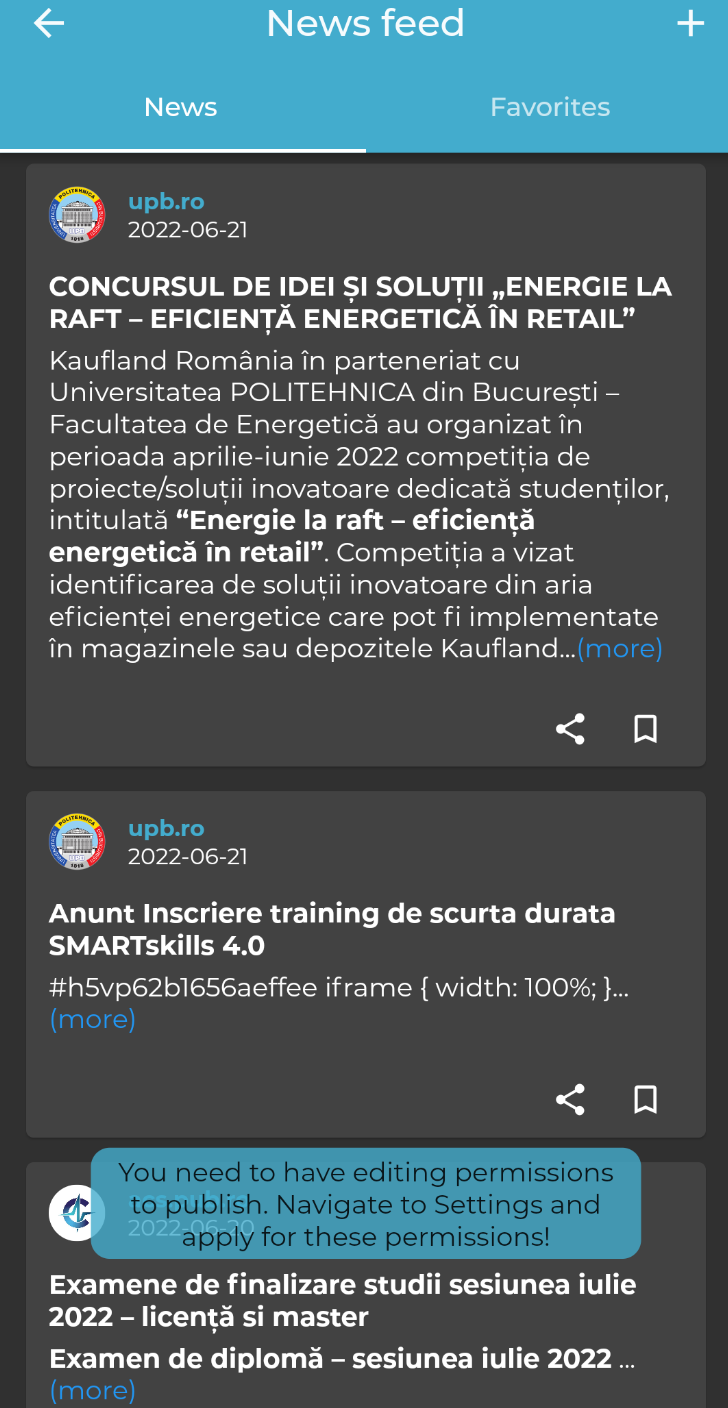
\includegraphics[width=\textwidth]{figures/app/final/news-feed-no-admin-final.png}
        \caption{User without editing permissions}
        \label{4:fig:user_no_permissions}
    \end{minipage}
    \hfill
    \begin{minipage}[b]{0.32\textwidth}
        \captionsetup{justification=centering}
        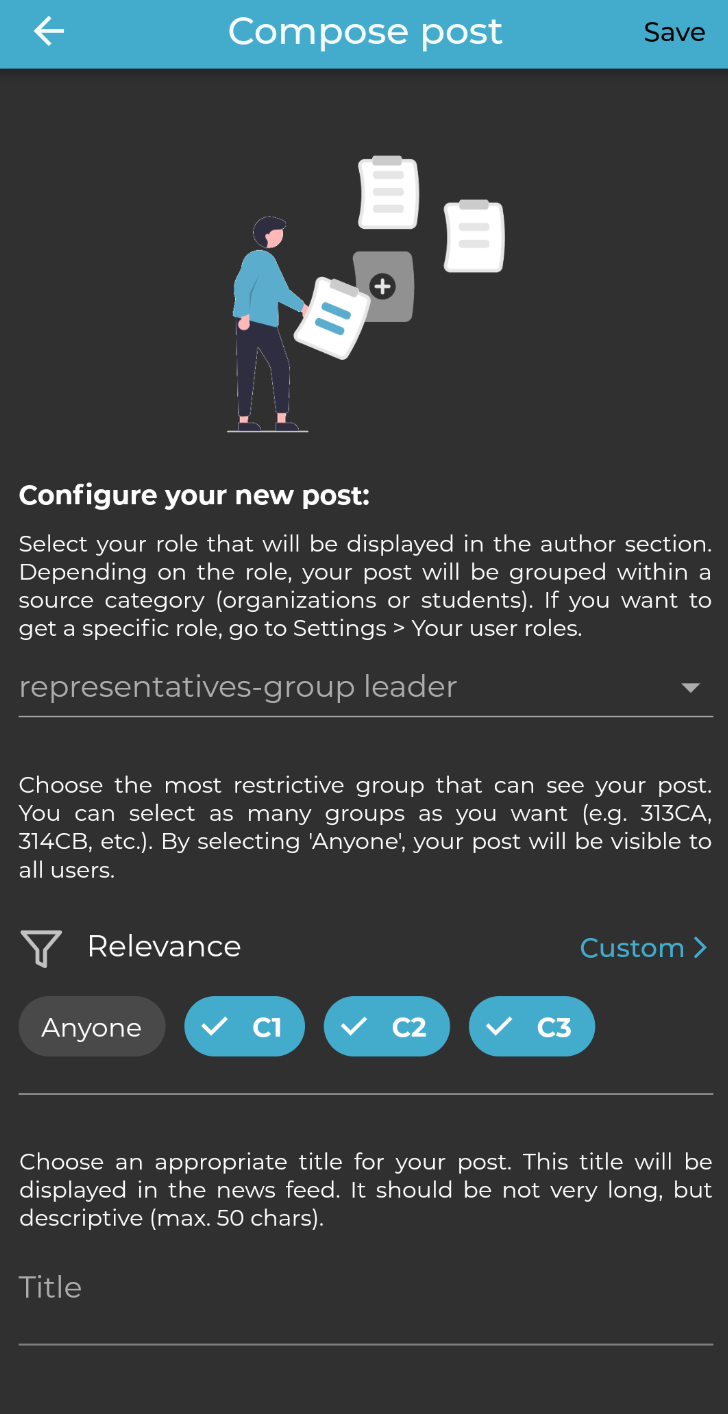
\includegraphics[width=\textwidth]{figures/app/final/compose-post-completion-1-final.png}
        \caption{Compose post page - 1}
        \label{4:fig:compose-post-1}
    \end{minipage}
    \hfill
    \begin{minipage}[b]{0.32\textwidth}
        \captionsetup{justification=centering}
        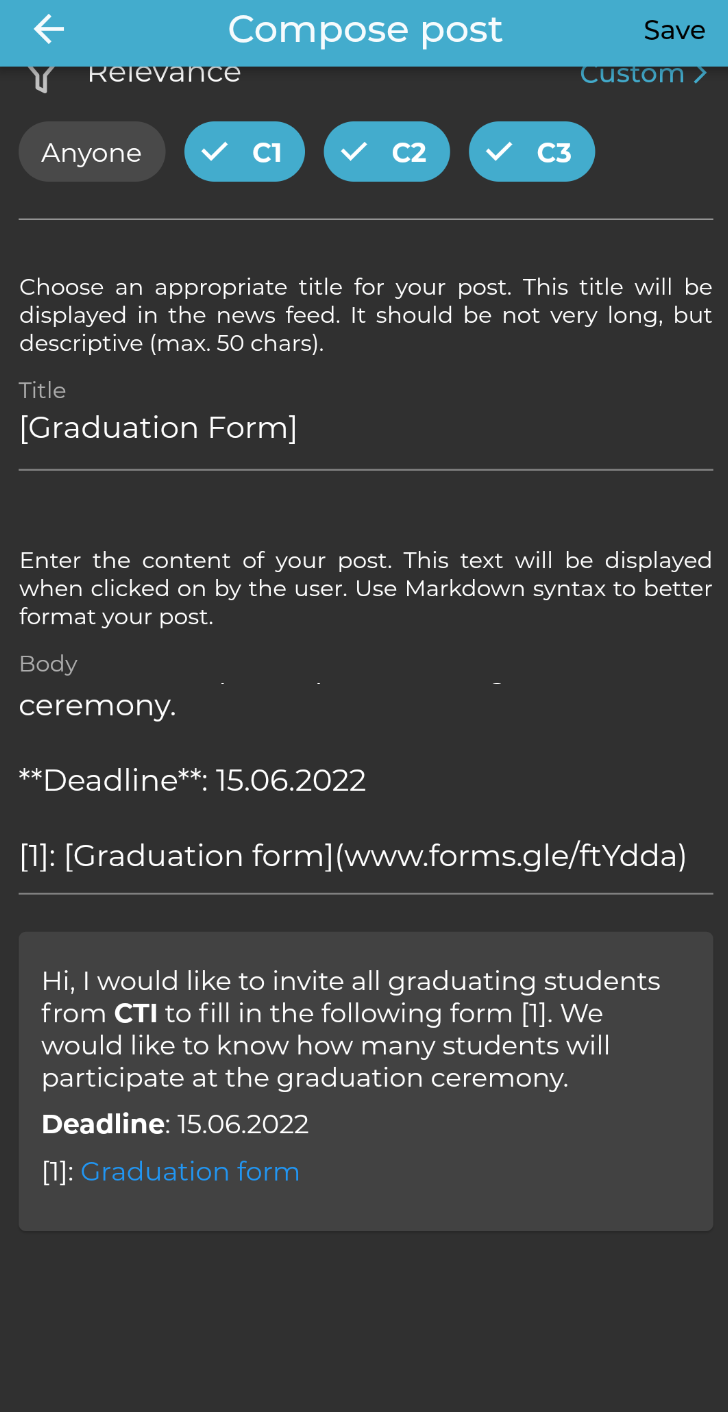
\includegraphics[width=\textwidth]{figures/app/final/compose-post-completion-2-final.png}
        \caption{Compose post page - 2}
        \label{4:fig:compose-post-2}
    \end{minipage}
\end{figure}

\begin{figure}[!ht]
    \centering
    \begin{minipage}[b]{0.32\textwidth}
        \captionsetup{justification=centering}
        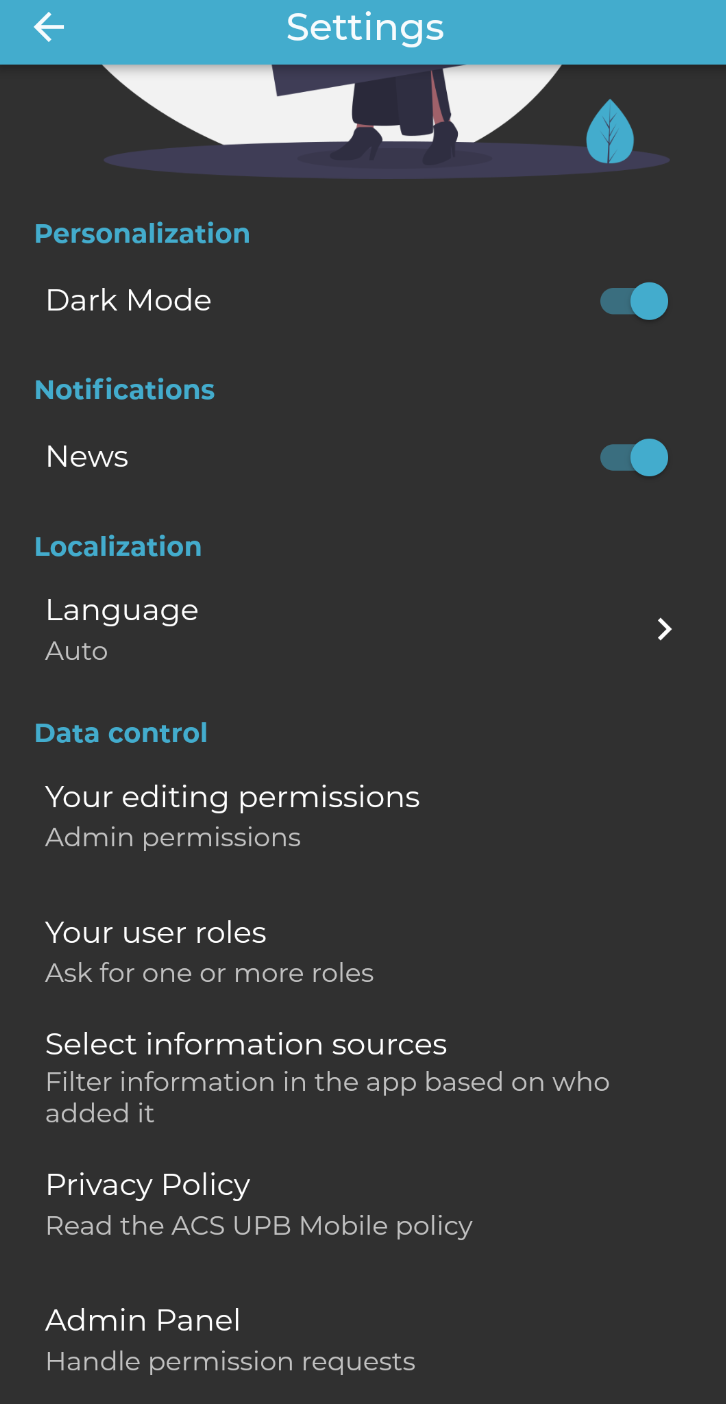
\includegraphics[width=\textwidth]{figures/app/final/settings-final.png}
        \caption{Settings main page}
        \label{4:fig:settings-page}
    \end{minipage}
    \hfill
    \begin{minipage}[b]{0.32\textwidth}
        \captionsetup{justification=centering}
        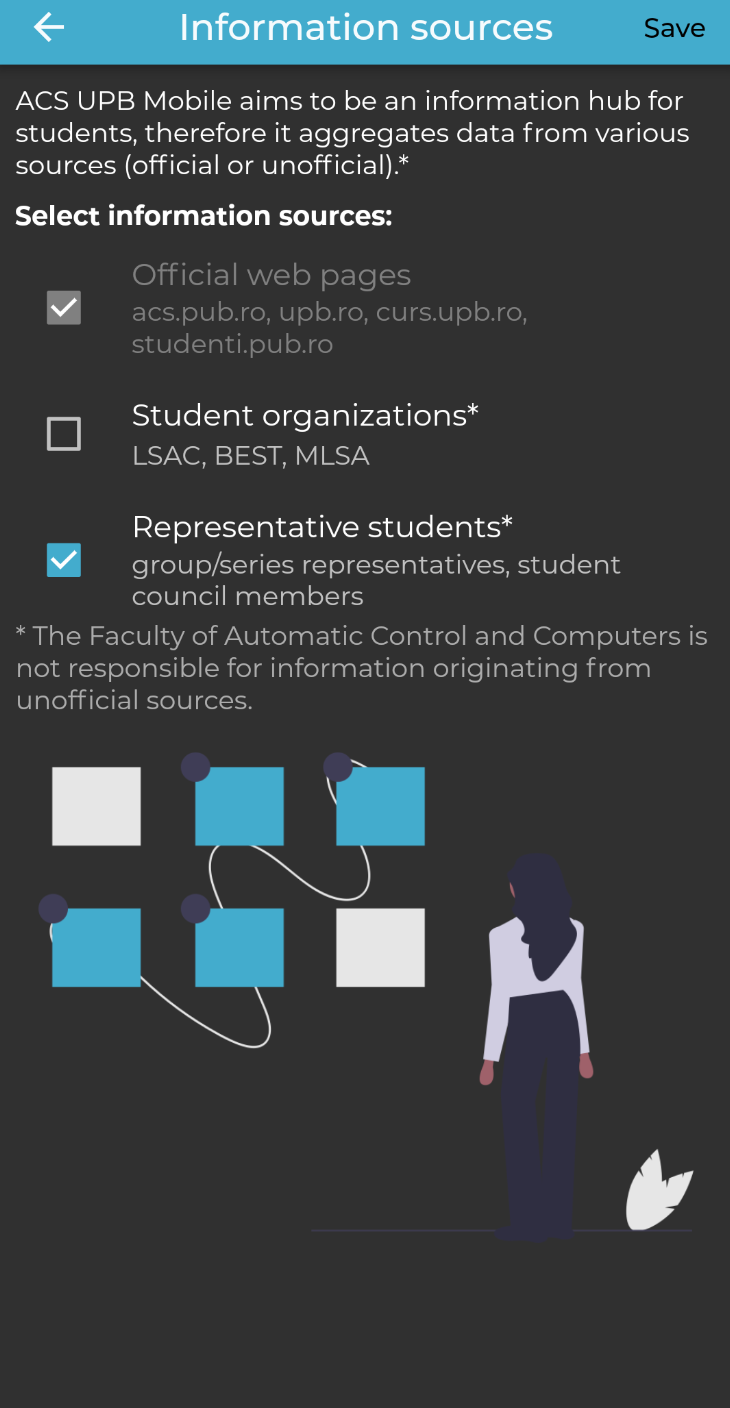
\includegraphics[width=\textwidth]{figures/app/final/select-sources-final.png}
        \caption{Select sources page}
        \label{4:fig:select_sources_page}
    \end{minipage}
    \hfill
    \begin{minipage}[b]{0.32\textwidth}
        \captionsetup{justification=centering}
        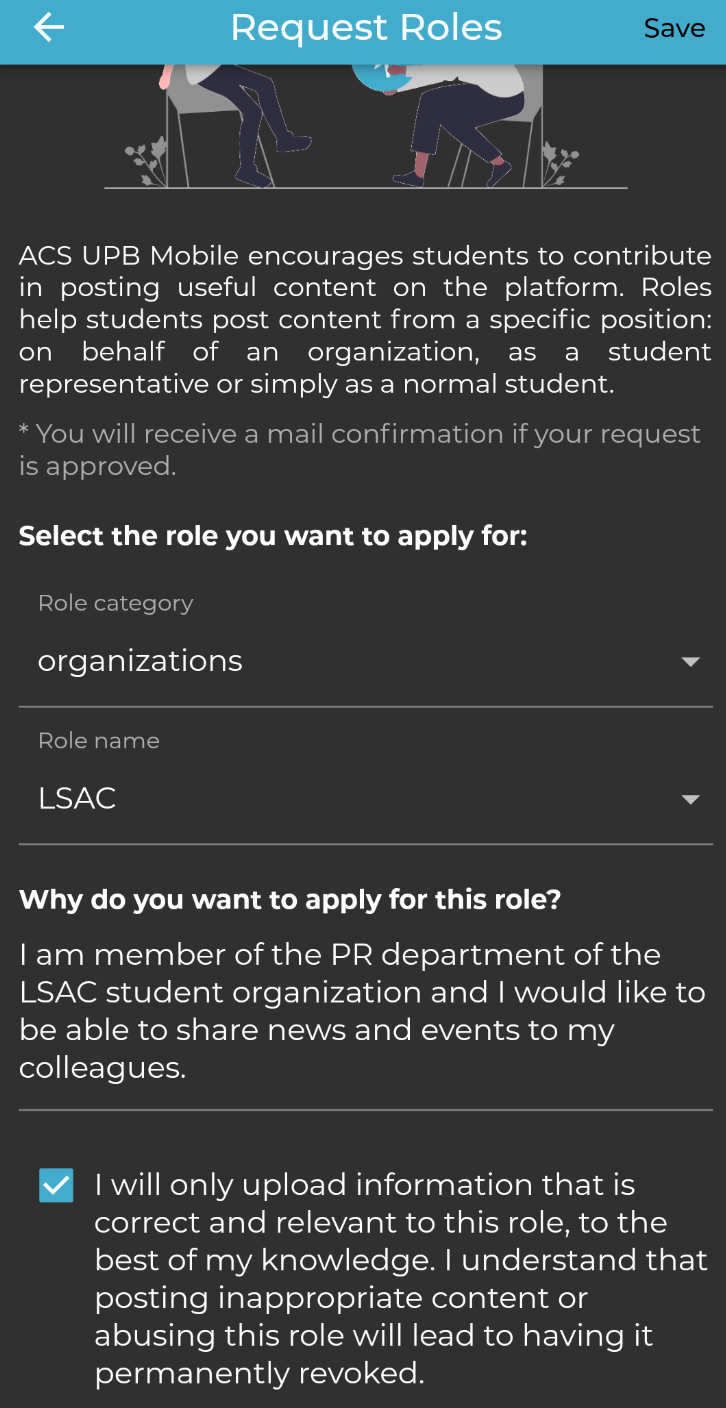
\includegraphics[width=\textwidth]{figures/app/final/request-roles-completed-final.png}
        \caption{Request roles form page}
        \label{4:fig:request-roles-completed-final}
    \end{minipage}
\end{figure}

~
We wanted the plus icon for adding a new post to be visible for all user types. When pressing on it, a normal user would receive a hint \textbf{\ref{4:fig:user_no_permissions}} to fill in a editing permissions request form by navigating to Settings \textbf{\ref{4:fig:settings-page}}. On the other hand, an Editor user is transitioned to a new page, where they can start publishing a new post. When composing a post, users choose a role, target group, title and body \textbf{\ref{4:fig:compose-post-1} \ref{4:fig:compose-post-2}.} \textbf{ACS UPB Mobile} can filter students based on their current year distribution (year, specialization, group, subgroup). We use the current architecture to target posts to one or more specific student groups. Editors can use Markdown syntax to give more expressiveness to their posts, and a live preview shows them exactly how the Markdown content is rendered.

~
Users navigate the settings and toggle the news slider to enable their notifications. When enabled, users receive notifications \textbf{\ref{4:fig:notifications-example}} whenever there is a new post available\footnote{notifications are currently available only on Android because iOS devices are more restrictive and require a developer license key}. Pressing on a notification would redirect the user to the news feed page \textbf{\ref{4:fig:news-feed-final}}. Furthermore, they can configure their information sources from the following settings page \textbf{\ref{4:fig:select_sources_page}}. When configuring their sources for the first time, users are directly prompted on successful login to this page, thus giving them the opportunity to select their information categories as early as possible. By default, users are subscribed to all categories because we wanted them to have access to all available information from the get-go.

~
When requesting roles \textbf{\ref{4:fig:request-roles-completed-final}} users need to select a role category, and a specific role name, and they must acknowledge the responsibilities of their actions. We took inspiration from the editing permissions request form already present in the app \textbf{\ref{4:fig:request-editing-permissions}}. Before applying for a publishing role, a user must acquire their editing permissions since we plan on giving restricted access to who can post content. After filling in a submission, an Admin reviews this application in the Admin Panel \textbf{\ref{4:fig:handle-requests}} and decides on accepting or declining it. This panel has two categories, one for editing permissions and the other for publishing roles. Upon accepting an application, the admin is redirected towards an emailing application to send the confirmation email to users. 

\begin{figure}[!ht]
    \centering
    \begin{minipage}[b]{0.32\textwidth}
        \captionsetup{justification=centering}
        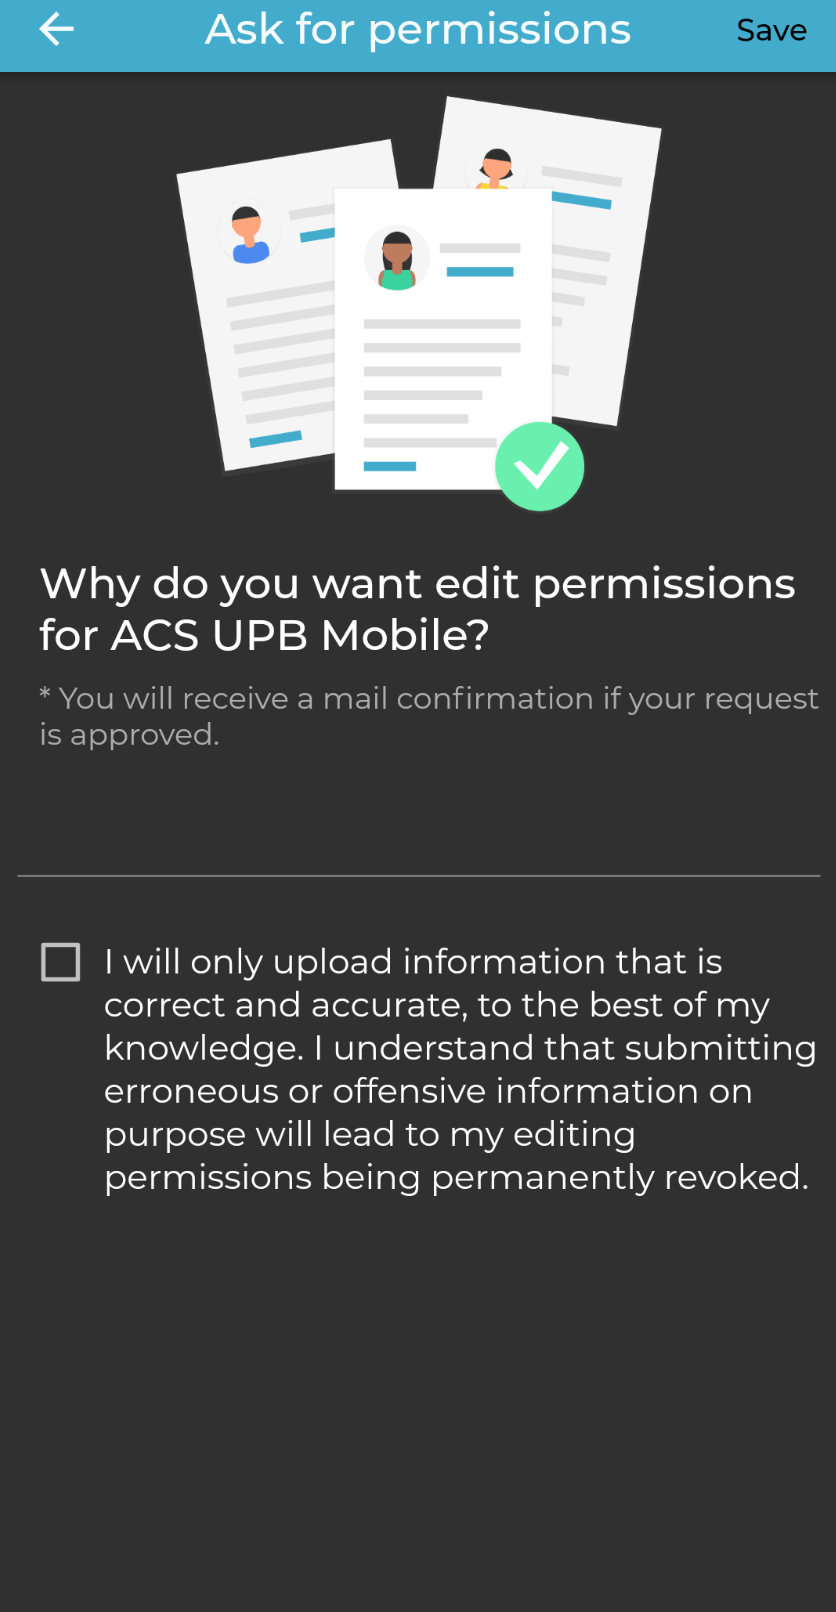
\includegraphics[width=\textwidth]{figures/app/final/request-editing-permissions.png}
        \caption{Editing permissions request form}
        \label{4:fig:request-editing-permissions}
    \end{minipage}
    \hfill
    \begin{minipage}[b]{0.32\textwidth}
        \captionsetup{justification=centering}
        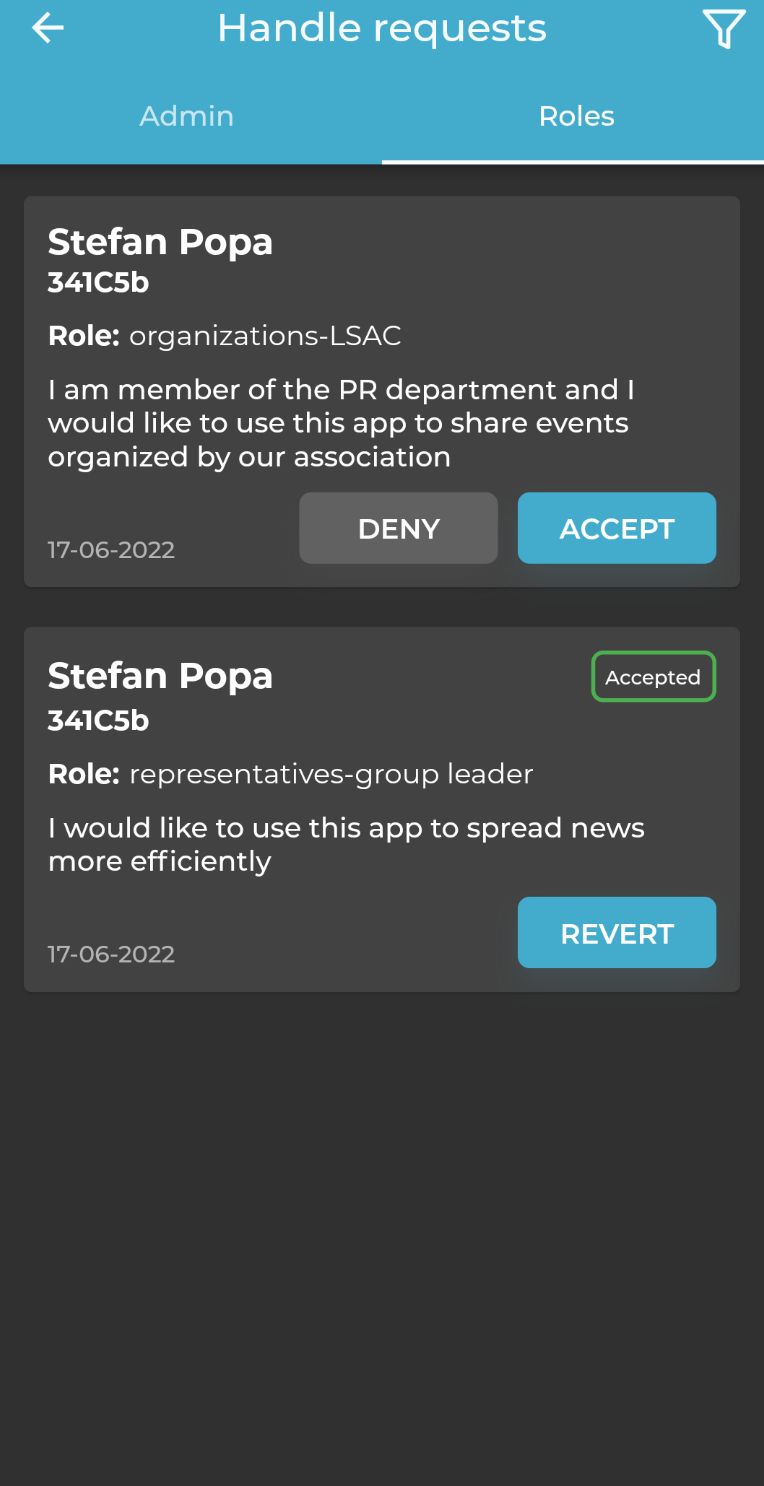
\includegraphics[width=\textwidth]{figures/app/final/handle-requests-completed-final.png}
        \caption{Admin panel for handling requests}
        \label{4:fig:handle-requests}
    \end{minipage}
    \hfill
    \begin{minipage}[b]{0.32\textwidth}
        \captionsetup{justification=centering}
        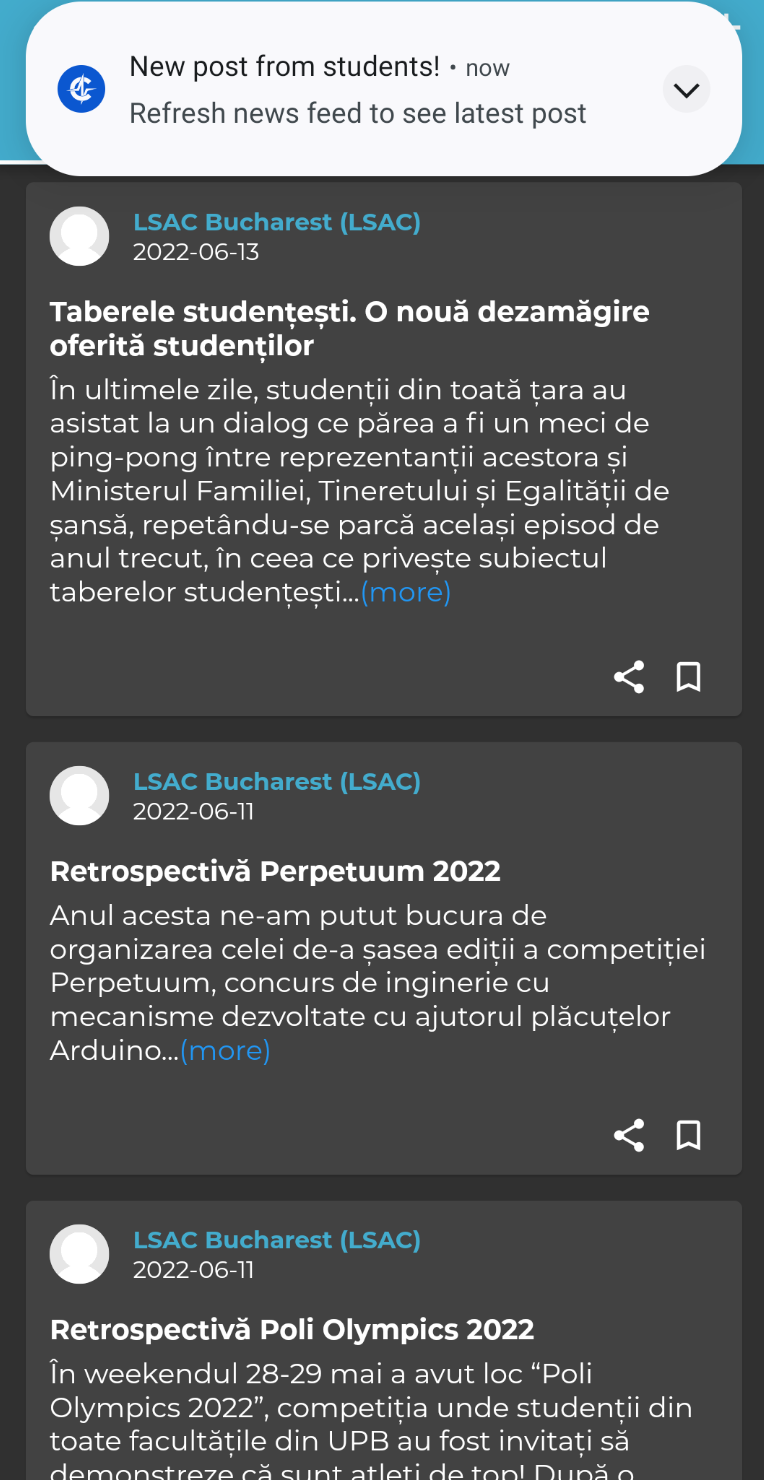
\includegraphics[width=\textwidth]{figures/app/final/new-post-students-final.png}
        \caption{Notifications example}
        \label{4:fig:notifications-example}
    \end{minipage}
\end{figure}
